\documentclass[11pt,letterpaper]{article}
\usepackage[margin=1in]{geometry}
\usepackage{fontspec}
\usepackage{xcolor}
\usepackage{tikz}
\usetikzlibrary{arrows.meta,positioning,shapes.geometric,fit,calc,decorations.pathreplacing}
\usepackage{booktabs}
\usepackage{tabularx}
\usepackage{hyperref}
\usepackage{parskip}
\usepackage{fancyhdr}

% Colors
\definecolor{cbblue}{HTML}{1E3A5F}
\definecolor{cblight}{HTML}{E8F0FE}
\definecolor{cborange}{HTML}{E67E22}
\definecolor{cbred}{HTML}{C0392B}
\definecolor{cbgreen}{HTML}{27AE60}
\definecolor{cbgray}{HTML}{7F8C8D}

\setmainfont{Helvetica Neue}[
  BoldFont = Helvetica Neue Bold,
  ItalicFont = Helvetica Neue Italic,
]

\hypersetup{
  colorlinks=true,
  linkcolor=cbblue,
  urlcolor=cbblue,
}

\pagestyle{fancy}
\fancyhf{}
\fancyhead[L]{\small\color{cbgray}ChatBridge — Pre-Search Document}
\fancyhead[R]{\small\color{cbgray}Gabriel Wilkins}
\fancyfoot[C]{\small\color{cbgray}\thepage}
\renewcommand{\headrulewidth}{0.4pt}

\begin{document}

% ─── Title ───────────────────────────────────────────────
\begin{center}
{\LARGE\bfseries\color{cbblue} ChatBridge}\\[4pt]
{\large Building an AI Chat Platform with Third-Party App Integration}\\[6pt]
{\normalsize Gabriel Wilkins \quad|\quad March 31, 2026}
\end{center}

\vspace{0.5em}
\noindent\rule{\textwidth}{0.5pt}
\vspace{0.5em}

% ─── Case Study Analysis ────────────────────────────────
\section*{Case Study Analysis}

TutorMeAI's competitive advantage isn't technology---it's trust. Ten thousand school
districts rely on them because teachers can shape the product to fit their classrooms.
The decision to open the platform to third-party apps threatens that trust at the exact
moment it could multiply it. The core tension: how do you let outside developers build
inside a product that serves children, without losing control of the experience those
children have?

The instinct is to lock everything down. Audit every app, sign every build, host
everything yourself. For a large district with a compliance department and budget,
that's the right answer. But most of TutorMeAI's ten thousand districts are small
schools where one administrator handles technology alongside everything else. A platform
that requires enterprise infrastructure to run safely isn't serving those schools. It's
excluding them.

We chose to build small and modular. Any school---public, private, charter, homeschool
co-op---can stand up ChatBridge and start using it. Teachers approve apps from a curated
catalog. The platform enforces safety at runtime through sandboxing, content filtering,
and audit logging, rather than requiring a pre-deployment review pipeline that small
organizations can't staff. This mirrors how education app stores already work: curate
at the gate, enforce at runtime, suspend instantly when something goes wrong.

The architectural decision that makes this tractable is treating third-party apps as
tools, not agents. Apps don't generate language or make decisions. They render UI and
hold state---a chess board, a weather dashboard, a vocabulary quiz. The AI is the only
thing that speaks to the student, and every word passes through content filtering before
it arrives. A malicious app can't say anything harmful to a child because it doesn't
speak. The attack surface collapses to what apps can display visually in their sandboxed
frame---which is why curation and runtime resource restrictions matter, but the problem
is a fraction of what it would be if apps could generate unrestricted text.

Content filtering for children isn't just catching bad words. A student typing ``I hate
my life'' requires a fundamentally different response than one typing profanity---the
platform has a duty of care to recognize crisis signals and alert a responsible adult
immediately, not just redact and log. We tier the filter pipeline: instant keyword
matching for the obvious, then a cheap fast classifier for intent and severity---
distinguishing frustration from crisis---with real-time alerts pushed to teachers
scaled by urgency. A teacher can kill a session or disable an app for their classroom
instantly, without waiting for a system administrator.

The ethical tradeoff we're making is explicit: we prioritize accessibility over maximum
control. An externally-hosted app can change what it serves after approval. We mitigate
this with runtime enforcement and instant suspension, but we cannot guarantee every pixel
a child sees. We believe this is the right tradeoff for the schools that need this
product most. Nothing in the architecture prevents a fully-audited managed hosting tier
from being added later---that's the path to serving districts that demand it. But the
foundation is built for the schools that would otherwise have nothing.

% ─── Technical Architecture ─────────────────────────────
\section*{Technical Architecture}

\subsection*{Stack Overview}

\begin{tabularx}{\textwidth}{l l X}
\toprule
\textbf{Layer} & \textbf{Choice} & \textbf{Rationale} \\
\midrule
Frontend & Chatbox fork (React 18) & Proven chat UI; strip Electron, keep renderer \\
Backend & Node 24 / Express & Handles auth, app registry, LLM proxy, safety \\
Database & PostgreSQL 16 & Multi-user concurrency, encrypted token storage \\
LLM & Vercel AI SDK & Already in Chatbox; multi-provider with middleware \\
Sandbox & Iframes + postMessage & Only real isolation for K-12 \\
Auth & JWT + OAuth2 proxy & Server holds all tokens; apps never see credentials \\
\bottomrule
\end{tabularx}

\vspace{0.5em}

Chatbox is a model-agnostic chat UI wrapper---message bubbles, streaming markdown,
provider configuration. No built-in safety, no system prompts. We keep the face,
replace the brain (server-side LLM with safety middleware) and the spine (PostgreSQL
instead of local storage).

\subsection*{Architecture Overview}

\begin{center}
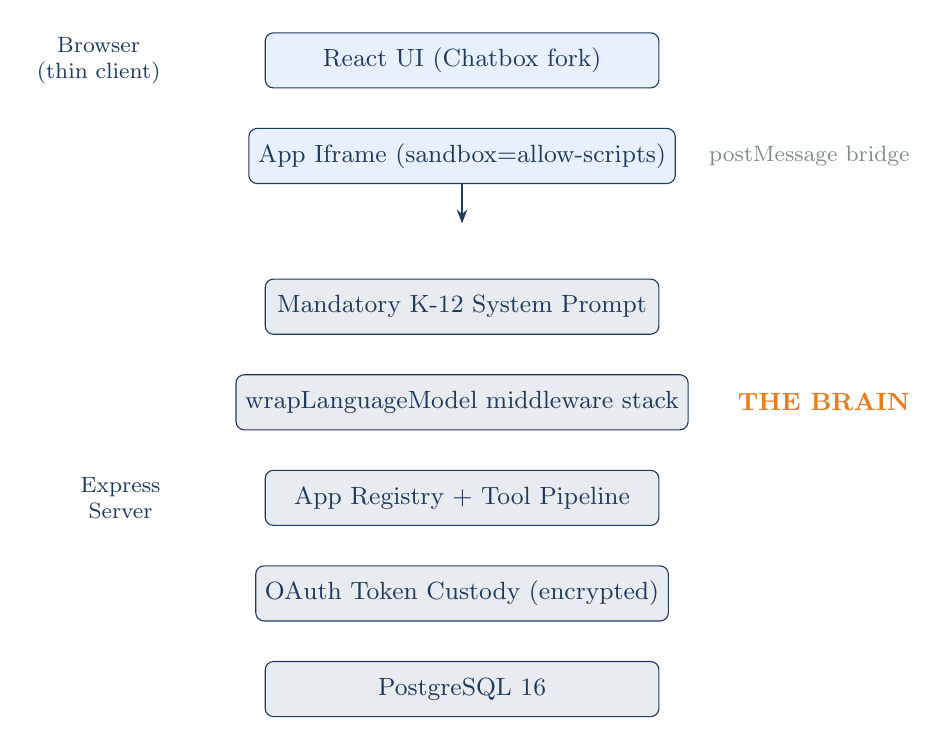
\begin{tikzpicture}[
  node distance=0.5cm,
  box/.style={rectangle, draw=cbblue, fill=cblight, rounded corners=3pt,
              minimum width=5cm, minimum height=0.7cm, font=\small,
              text=cbblue, align=center},
  serverbox/.style={rectangle, draw=cbblue, fill=cbblue!10, rounded corners=3pt,
              minimum width=5cm, minimum height=0.7cm, font=\small,
              text=cbblue, align=center},
  sidelabel/.style={font=\footnotesize\color{cbgray}, align=right},
  arrow/.style={-{Stealth[length=5pt]}, thick, cbblue},
  brace/.style={decorate, decoration={brace, amplitude=6pt, raise=2pt}, thick, cbblue},
]

% Browser side
\node[box] (ui) {React UI (Chatbox fork)};
\node[box, below=of ui] (iframe) {App Iframe (sandbox=allow-scripts)};
\node[right=0.3cm of iframe, font=\footnotesize\color{cbgray}] {postMessage bridge};

% Browser group label
\node[left=1.2cm of ui, font=\footnotesize\color{cbblue}, align=center] (browserlabel) {Browser\\(thin client)};

% Arrow to server
\draw[arrow] (iframe.south) -- ++(0,-0.5);

% Server side
\node[serverbox, below=1.2cm of iframe] (prompt) {Mandatory K-12 System Prompt};
\node[serverbox, below=of prompt] (middleware) {wrapLanguageModel middleware stack};
\node[serverbox, below=of middleware] (registry) {App Registry + Tool Pipeline};
\node[serverbox, below=of registry] (custody) {OAuth Token Custody (encrypted)};
\node[serverbox, below=of custody] (db) {PostgreSQL 16};

% Server group label
\node[left=1.2cm of registry, font=\footnotesize\color{cbblue}, align=center] {Express\\Server};

% Label the server as the brain
\node[right=0.5cm of middleware, font=\small\bfseries\color{cborange}] {THE BRAIN};

\end{tikzpicture}
\end{center}

% ─── Safety Architecture Diagram ────────────────────────
\subsection*{Trust \& Safety Architecture}

Apps are tools, not agents. They can't generate language---only the LLM speaks to
the student. This collapses the app threat model to two vectors:

\begin{center}
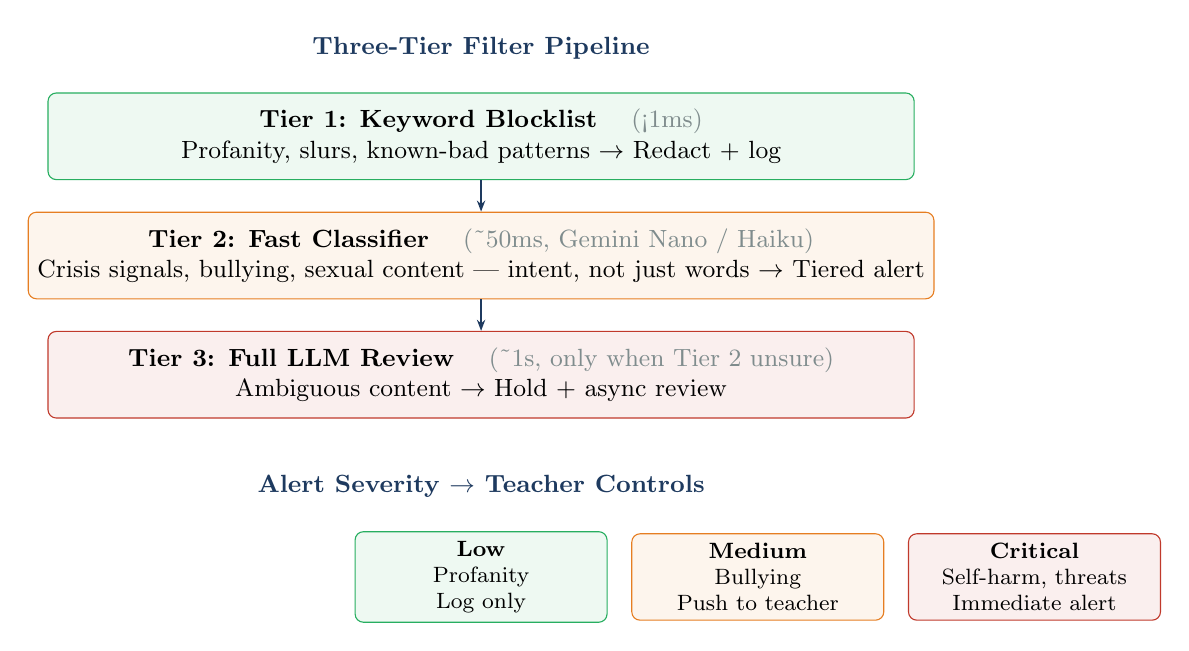
\begin{tikzpicture}[
  node distance=0.4cm and 1cm,
  tier/.style={rectangle, draw=#1, fill=#1!8, rounded corners=3pt,
               minimum width=11cm, minimum height=1.1cm, font=\small,
               align=center},
  severity/.style={rectangle, draw=#1, fill=#1!8, rounded corners=3pt,
               minimum width=3.2cm, minimum height=0.9cm, font=\footnotesize,
               align=center},
  heading/.style={font=\small\bfseries\color{cbblue}},
]

% Filter Pipeline
\node[heading] (fh) {Three-Tier Filter Pipeline};
\node[tier=cbgreen, below=0.3cm of fh] (t1) {
  \textbf{Tier 1: Keyword Blocklist} \quad {\color{cbgray}(<1ms)} \\
  Profanity, slurs, known-bad patterns $\rightarrow$ Redact + log
};
\node[tier=cborange, below=of t1] (t2) {
  \textbf{Tier 2: Fast Classifier} \quad {\color{cbgray}(\textasciitilde50ms, Gemini Nano / Haiku)} \\
  Crisis signals, bullying, sexual content --- intent, not just words $\rightarrow$ Tiered alert
};
\node[tier=cbred, below=of t2] (t3) {
  \textbf{Tier 3: Full LLM Review} \quad {\color{cbgray}(\textasciitilde1s, only when Tier 2 unsure)} \\
  Ambiguous content $\rightarrow$ Hold + async review
};

% Severity levels
\node[heading, below=0.6cm of t3] (sh) {Alert Severity $\rightarrow$ Teacher Controls};

\node[severity=cbgreen, below=0.3cm of sh] (s1) {\textbf{Low}\\Profanity\\Log only};
\node[severity=cborange, right=0.3cm of s1] (s2) {\textbf{Medium}\\Bullying\\Push to teacher};
\node[severity=cbred, right=0.3cm of s2] (s3) {\textbf{Critical}\\Self-harm, threats\\Immediate alert};

% Arrows
\draw[-{Stealth[length=4pt]}, thick, cbblue] (t1.south) -- (t2.north);
\draw[-{Stealth[length=4pt]}, thick, cbblue] (t2.south) -- (t3.north);

\end{tikzpicture}
\end{center}

\vspace{0.3em}

\noindent\textbf{Defense in depth (4 layers):}

\begin{tabularx}{\textwidth}{l X}
\toprule
\textbf{Iframe sandbox} & \texttt{allow-scripts} only. No same-origin, no navigation, no popups. App cannot access platform DOM, cookies, or storage. \\
\midrule
\textbf{Content filter} & Every LLM token and every tool result passes through the three-tier pipeline before reaching the student. \\
\midrule
\textbf{Curated registry} & Teachers/admins approve apps. Report + instant platform-wide suspend. \\
\midrule
\textbf{Data isolation} & Apps can't read other apps' data or conversation history. OAuth tokens encrypted at rest, never sent to iframes. \\
\bottomrule
\end{tabularx}

% ─── Tool Invocation Lifecycle ──────────────────────────
\subsection*{Tool Invocation Lifecycle}

\begin{center}
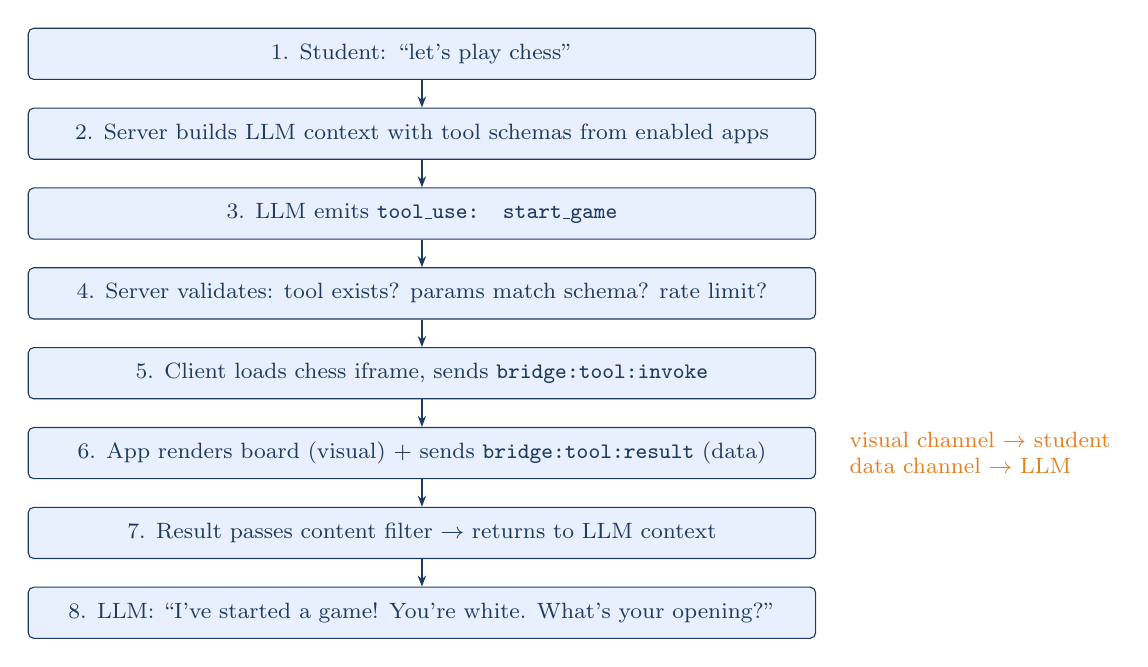
\begin{tikzpicture}[
  node distance=0.35cm,
  flowstep/.style={rectangle, draw=cbblue, fill=cblight, rounded corners=2pt,
               minimum width=10cm, minimum height=0.65cm, font=\footnotesize,
               text=cbblue, align=left},
  arrow/.style={-{Stealth[length=4pt]}, thick, cbblue},
]

\node[flowstep] (s1) {1. Student: ``let's play chess''};
\node[flowstep, below=of s1] (s2) {2. Server builds LLM context with tool schemas from enabled apps};
\node[flowstep, below=of s2] (s3) {3. LLM emits \texttt{tool\_use: start\_game}};
\node[flowstep, below=of s3] (s4) {4. Server validates: tool exists? params match schema? rate limit?};
\node[flowstep, below=of s4] (s5) {5. Client loads chess iframe, sends \texttt{bridge:tool:invoke}};
\node[flowstep, below=of s5] (s6) {6. App renders board (visual) + sends \texttt{bridge:tool:result} (data)};
\node[flowstep, below=of s6] (s7) {7. Result passes content filter $\rightarrow$ returns to LLM context};
\node[flowstep, below=of s7] (s8) {8. LLM: ``I've started a game! You're white. What's your opening?''};

\foreach \i/\j in {s1/s2, s2/s3, s3/s4, s4/s5, s5/s6, s6/s7, s7/s8} {
  \draw[arrow] (\i.south) -- (\j.north);
}

% Dual channel annotation
\node[right=0.3cm of s6, font=\footnotesize\color{cborange}, align=left]
  {visual channel $\rightarrow$ student\\data channel $\rightarrow$ LLM};

\end{tikzpicture}
\end{center}

\noindent\textbf{Resilience:} 30-second timeout per invocation. Circuit breaker auto-disables
an app after 3 failures in 5 minutes. Graceful error messages back to the LLM.

% ─── Three-Loop Architecture ────────────────────────────
\subsection*{Three-Loop Agent Architecture}

\begin{center}
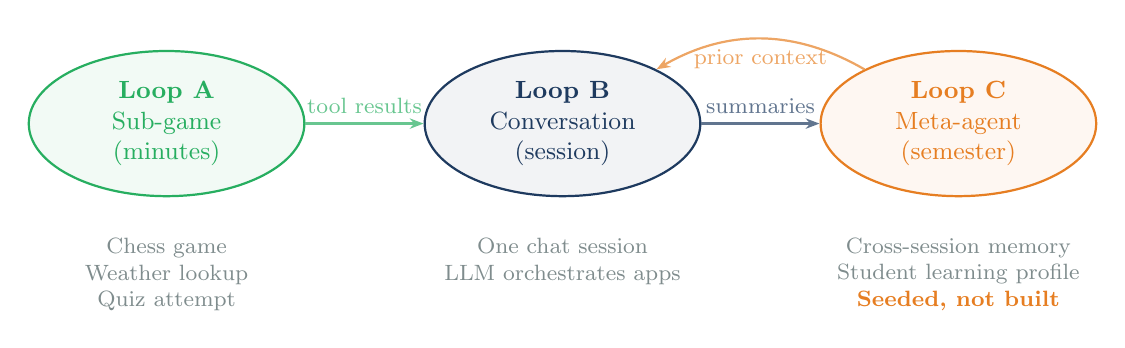
\begin{tikzpicture}[
  loop/.style={ellipse, draw=#1, thick, fill=#1!6, minimum width=3.5cm,
               minimum height=1.8cm, font=\small, align=center, text=#1},
]

\node[loop=cbgreen] (a) {\textbf{Loop A}\\Sub-game\\(minutes)};
\node[loop=cbblue, right=1.5cm of a] (b) {\textbf{Loop B}\\Conversation\\(session)};
\node[loop=cborange, right=1.5cm of b] (c) {\textbf{Loop C}\\Meta-agent\\(semester)};

\draw[-{Stealth[length=5pt]}, thick, cbgreen!70] (a) -- (b)
  node[midway, above, font=\footnotesize\color{cbgray}] {tool results};
\draw[-{Stealth[length=5pt]}, thick, cbblue!70] (b) -- (c)
  node[midway, above, font=\footnotesize\color{cbgray}] {summaries};
\draw[-{Stealth[length=5pt]}, thick, cborange!70, bend right=30] (c) to
  node[midway, below, font=\footnotesize\color{cbgray}] {prior context} (b);

\node[below=0.4cm of a, font=\footnotesize\color{cbgray}, align=center]
  {Chess game\\Weather lookup\\Quiz attempt};
\node[below=0.4cm of b, font=\footnotesize\color{cbgray}, align=center]
  {One chat session\\LLM orchestrates apps};
\node[below=0.4cm of c, font=\footnotesize\color{cbgray}, align=center]
  {Cross-session memory\\Student learning profile\\{\color{cborange}\textbf{Seeded, not built}}};

\end{tikzpicture}
\end{center}

% ─── App Integration Patterns ───────────────────────────
\subsection*{Three App Integration Patterns}

\begin{tabularx}{\textwidth}{l l l X}
\toprule
\textbf{App} & \textbf{Trust Tier} & \textbf{Auth} & \textbf{Demonstrates} \\
\midrule
Chess & Internal & None & Complex bidirectional state, ongoing interaction \\
Wordle & External Public & Proxied dictionary API & Word validation via \texttt{bridge:api:request}, session game \\
Vocab Quiz & Internal & None & Educational content delivery, LLM-mediated Q\&A \\
\bottomrule
\end{tabularx}

% ─── Session Lifecycle ──────────────────────────────────
\subsection*{Session Lifecycle}

When a conversation approaches context window limits: graceful wind-down with
LLM-generated structured summary (topics, apps used, outcomes) stored in PostgreSQL.
Full transcript retained in the \texttt{messages} table---the LLM can query its own
conversation history as a tool if it needs specifics the summary lost. Compact the
context, keep the record.

% ─── Design Decision ────────────────────────────────────
\subsection*{Key Design Decision: Accessibility Over Maximum Control}

We optimize for small schools and open-source deployments. Apps are hosted externally
by their developers, not audited and served from our infrastructure. The curated
registry, runtime sandboxing, and content filtering provide the safety floor. Nothing
in the architecture prevents adding a managed, fully-audited hosting tier later---the
trust tier system is designed to extend. ChatBridge starts as something any school can
stand up. A SaaS vendor can build an enterprise version with per-district plugin
verification on top of the same architecture.

% ─── Constraints ───────────────────────────────────────
\section*{Constraints}

\begin{tabularx}{\textwidth}{l X}
\toprule
\textbf{Constraint} & \textbf{Impact} \\
\midrule
Solo + AI agents & One person coordinating multiple Claude Code instances. Tasks must be agent-sized (3--8 files, one concern, clear entry/exit). No pair programming. \\
One-week sprint & Scope must be ruthlessly vertical. Ship working slices, not horizontal layers. \\
Fork of Chatbox & Inherit React 18, Mantine, Vite, Zustand/Jotai. Can't choose the frontend stack---must strip Electron and build on what's there. \\
K-12 audience & Trust \& safety is load-bearing architecture, not a feature. Content filtering, audit logging, and teacher controls are on the critical path, not nice-to-haves. \\
Small-school target & Can't assume enterprise infra: no signing pipelines, no CDN, no dedicated IT staff. Must work on a single VPS. \\
\bottomrule
\end{tabularx}

% ─── Alternatives Considered ──────────────────────────
\section*{Alternatives Considered}

\subsection*{App Sandbox: Iframes vs.\ Web Components vs.\ Server-Side Rendering}

\begin{tabularx}{\textwidth}{l l X}
\toprule
\textbf{Option} & \textbf{Isolation} & \textbf{Assessment} \\
\midrule
\textbf{Iframes} {\color{cbgreen}(chosen)} & Process-level & Real security boundary. \texttt{sandbox} attribute strips DOM access, navigation, popups. Only option that provides actual isolation for K-12. \\
Web Components & DOM-level & Shadow DOM is encapsulation, not security. A malicious component can still access \texttt{window}, \texttt{document}, cookies. Insufficient for children's product. \\
Server-side render & Full & App runs on server, sends HTML. Maximum control but kills interactivity (chess board, real-time games). Latency on every interaction. \\
\bottomrule
\end{tabularx}

\subsection*{App Hosting: External vs.\ Managed}

\begin{tabularx}{\textwidth}{l X}
\toprule
\textbf{Option} & \textbf{Assessment} \\
\midrule
\textbf{External iframes} {\color{cbgreen}(chosen)} & Apps hosted by developers, loaded via iframe. Platform controls access through curated registry, sandbox, CSP. Any school can deploy without signing infrastructure. Any developer can build an app. \textbf{Risk:} approved app can change after approval. \textbf{Mitigation:} runtime enforcement + instant suspend. \\
Signed/managed & Apps audited, signed, served from platform CDN. Guarantees content integrity. Requires review pipeline, hosting infra, and ongoing labor that small schools can't provide. Kills third-party adoption. \\
\bottomrule
\end{tabularx}

\noindent\textit{Nothing in the architecture prevents adding a managed tier later---the trust tier system is designed to extend. We start accessible.}

\subsection*{Content Filtering: Keywords vs.\ Classifier vs.\ Tiered}

\begin{tabularx}{\textwidth}{l X}
\toprule
\textbf{Option} & \textbf{Assessment} \\
\midrule
Keywords only & Fast, cheap, no false positives on exact matches. Misses intent entirely. ``I want to die'' vs ``I want to die laughing.'' Unacceptable for K-12. \\
Classifier only & Understands intent but adds latency (\textasciitilde50ms) and cost to every message. Overkill for obvious profanity. \\
\textbf{Tiered pipeline} {\color{cbgreen}(chosen)} & Keywords first (<1ms), classifier second (only when needed), full review third (only when uncertain). Each tier catches what the previous misses. Cost scales with risk, not volume. \\
\bottomrule
\end{tabularx}

\subsection*{LLM Integration: Client-Side vs.\ Server-Mediated}

\begin{tabularx}{\textwidth}{l X}
\toprule
\textbf{Option} & \textbf{Assessment} \\
\midrule
Client-side (Chatbox default) & User configures API key, calls go direct. No content filtering possible, no audit trail, no mandatory system prompt. Chatbox trusts the user---but our users are children. \\
\textbf{Server-mediated} {\color{cbgreen}(chosen)} & All LLM calls through Express backend. Enables mandatory safety middleware, tool pipeline orchestration, audit logging, cost tracking. The server is the brain; the frontend is a thin streaming client. \\
\bottomrule
\end{tabularx}

% ─── Build Order ──────────────────────────────────────
\section*{Build Order \& Timeline}

One-week sprint. Solo developer with AI coding agents running in parallel.

\begin{enumerate}
  \item \textbf{Day 1 (Mon):} Fork Chatbox, strip Electron. Scaffold Express backend, PostgreSQL schema, shared types. Three agents in parallel.
  \item \textbf{Day 2 (Tue):} User auth (JWT). Chat API with streaming. Content safety middleware. Presearch document + architecture video.
  \item \textbf{Day 3 (Wed):} App registry + manifest validation. Bridge protocol + iframe host. Tool pipeline integration---\textit{the crux}, where all three subsystems meet.
  \item \textbf{Day 4 (Thu):} Chess app (required). Second app. Third app. Deploy to Linode. Early submission.
  \item \textbf{Day 5--7 (Fri--Sun):} OAuth app, conversation summaries (Loop C seed), developer docs, polish, final submission.
\end{enumerate}

\noindent\textbf{Critical path:} Fork $\rightarrow$ Server + DB + Types (parallel) $\rightarrow$ Auth + Chat API $\rightarrow$ Safety + Registry + Bridge (parallel) $\rightarrow$ Tool Pipeline $\rightarrow$ Apps (parallel).

\noindent\textbf{Parallelization:} After the tool pipeline integrates, all apps and deployment can run simultaneously in separate agent sessions.

% ─── Risk Analysis ────────────────────────────────────
\section*{Risk Analysis}

\begin{tabularx}{\textwidth}{X c X}
\toprule
\textbf{Risk} & \textbf{Severity} & \textbf{Mitigation} \\
\midrule
LLM ignores tools and fabricates game results instead of calling app & High & Strong system prompt with explicit tool routing per app. Idempotent \texttt{start\_game} guards prevent state resets. Larger models far more reliable than mini. \\
\addlinespace
Iframe renders inappropriate visual content that platform cannot inspect & Medium & Curated registry with teacher approval gate. Iframe CSP restricts loadable resources. Report + instant platform-wide suspend. \\
\addlinespace
Context window overflow in long multi-app conversations & Medium & \texttt{stepCountIs(5)} limits tool rounds per message. Context builder manages schema injection. Future: conversation compaction. \\
\addlinespace
Approved app changes behavior after approval (supply chain) & Medium & Runtime enforcement: sandbox + content filter on all tool results before LLM context. Instant suspend on report. Trust tier system extensible to managed hosting. \\
\addlinespace
One-week timeline for full-stack platform & High & Vertical slices over horizontal layers. Ship working chat + one app before adding more. AI agent parallelization on clean module seams. \\
\bottomrule
\end{tabularx}

% ─── Validation Plan ──────────────────────────────────
\section*{Validation \& Testing Plan}

Seven scenarios from the PRD, mapped to verification approach:

\begin{tabularx}{\textwidth}{r X l}
\toprule
\textbf{\#} & \textbf{Scenario} & \textbf{Method} \\
\midrule
1 & Tool discovery and invocation & Live demo: ``let's play chess'' \\
2 & App UI renders in chat & Live demo: board/quiz card appears \\
3 & User interacts, completion signaling & Live demo: moves/guesses via bridge \\
4 & Context retention after app interaction & Ask ``what did I get wrong?'' \\
5 & Switch between multiple apps & Wordle $\rightarrow$ Quiz in one conversation \\
6 & Ambiguous routing accuracy & Natural language $\rightarrow$ correct app \\
7 & Refuses to invoke for unrelated queries & Normal question gets text answer \\
\bottomrule
\end{tabularx}

\noindent\textbf{Safety validation:} Type flagged content as student, verify real-time appearance on teacher safety dashboard with correct severity classification. Test keyword tier (profanity) and classifier tier (threats without keywords) independently.

\noindent\textbf{Observability:} Every tool invocation logged to \texttt{tool\_invocations} table with parameters, result, status, and duration. Content filter matches logged to \texttt{content\_filter\_log} with severity, source, and matched words. Teacher dashboard provides runtime verification.

\end{document}
